\begin{pastexam}[label={px:ntust-113-ice-08}]{臺科大資工所 113 學年度 第 II-2 題}
（填充）

II.\quad \underline{(65\%) Fill in the following blanks.}

(5\%) There are three types of iterative binary tree traversal (i.e., inorder, preorder, and
postorder). Conduct a traversal of the following binary tree using preorder. What is the 5th element
of this preorder traversal? \blank{C}
\begin{center}
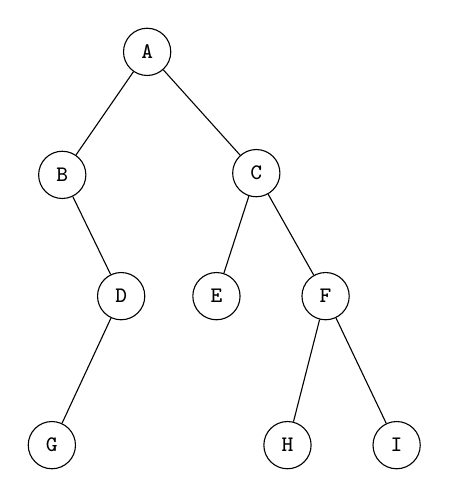
\begin{tikzpicture}[x=0.022cm,y=-0.022cm,every node/.style={circle,draw,inner sep=0pt,minimum size=6mm,font=\ttfamily\footnotesize}]
\node (A) at (490,676) {A};
\node (B) at (441,747) {B};
\node (C) at (553,746) {C};
\node (D) at (475,817) {D};
\node (E) at (530,817) {E};
\node (F) at (593,817) {F};
\node (G) at (435,903) {G};
\node (H) at (571,903) {H};
\node (I) at (634,903) {I};
\draw (A)--(B) (A)--(C) (B)--(D) (C)--(E) (C)--(F) (D)--(G) (F)--(H) (F)--(I);
\end{tikzpicture}
\end{center}
\end{pastexam}

\begin{pastsoln}
答案：(C) 填 C。

先讀出樹的結構：A 的左、右子節點是 B、C；B 只有\textbf{右}子節點 D；D 只有\textbf{左}子節點 G；
C 的左、右子節點是 E、F；F 的左、右子節點是 H、I。 前序是「根、左子樹、右子樹」（資結書
第~7.3~節）：
\begin{enumerate}
\item A（根）
\item B（A 的左子樹的根）；B 沒有左子樹，接著走右子樹
\item D
\item G（D 的左子節點）；B 的子樹走完，回到 A 的右子樹
\item \textbf{C}
\item E
\item F
\item H
\item I
\end{enumerate}
前序是 A, B, D, G, C, E, F, H, I，第 $5$ 個是 C。 （這題 D 在左或右不影響前序，因為 B 只有一個
子節點；但中序、後序就會受影響。）
\end{pastsoln}
